% This is LLNCS.DEM the demonstration file of
% the LaTeX macro package from Springer-Verlag
% for Lecture Notes in Computer Science,
% version 2.4 for LaTeX2e as of 16. April 2010
%
\documentclass{article}
%
\usepackage{makeidx}  % allows for indexgeneration
\usepackage{color} %vrivas, 15-Jan-2016
\usepackage{hyperref} %vrivas, 21-Jan-2016, for \url
\usepackage{graphicx} %vrivas, 27-Jan-2016, for images
\usepackage{listings}%vrivas, 27-Jan-2016, for code
\usepackage{algorithm} %jj, dec-8-2016, for code
\usepackage{algorithmic} %jj, dec-8-2016, for code
\usepackage{authblk} %jj, dec-20-2016, for authors

\begin{document}
%


\title{Time series forecasting using evolutionary neural nets implemented in a
  volunteer computing system}

% Author according to authblk
\author[1,4]{V.M. Rivas}
\author[1]{E. Parras-Guti\'{e}rrez}
\author[2,4]{JJ Merelo}
\author[2,4]{M.G. Arenas}
\author[3,4]{P. Garc\'{\i}a-Fern\'{a}ndez}

% Affiliations according to authblk
\affil[1]{Univ. of Jaen, Dept of Computer Sciences,\\
Campus Las Lagunillas s/n, 23071, Ja\'{e}n, SPAIN\\
\texttt{vrivas@ujaen.es},
\texttt{http://vrivas.es}}

\affil[2]{%Depto. de Arquitectura y Tecnolog\'{\i}as de las Computadoras\\
%Univ. de Granada, SPAIN
Univ. of Granada, Dept. of Computers, Architecture and Technology\\
C/ Periodista Daniel Saucedo s/n, 18071, Granada, SPAIN}

\affil[3]{%Depto. de Electr\'{o}nica y Tecnolog\'{\i}as de las
  %Computadoras\\
 %Univ. de Granada, SPAIN
 Univ. of Granada, Dept. of Electronics and Computer Technology\\
C/ Periodista Daniel Saucedo s/n, 18071, Granada, SPAIN}


\affil[4]{GeNeura Team \\
  \url{http://geneura.wordpress.com}
}

\maketitle              % typeset the title of the contribution
\begin{abstract}
%##### NUEVA PROPUESTA DE ABSTRACT--- Maribel
% Victor: Ojo: m�ximo 100 palabras seg�n las normas de la publicaci�n
% http://onlinelibrary.wiley.com/journal/10.1002/(ISSN)1099-1174/homepage/ForAuthors.html
{\em jsEvRBF} is a time-series forecasting method based on genetic algorithm
and neural nets. Written in JavaScript language, can be executed in most web browsers.
Consequently, everybody can participate in the experiments, and
scientists can take advantage of nowadays available browsers and devices as computation environments. 
This is also a great challenge
as the language support and performance varies from one browser to another.
In this paper, {\em jsEvRBF} has been tested in a volunteer computing experiment, and also in a single-browser one.
Both experiments are related to forecasting currencies exchange, and the results show the viability of the proposal.

%#### cuando tengamos nuevos resultados puedo concretar un poco m �s la �ltima frase, que la he dejado un poco ambig�a
% You can't say "the presented results do this". Say what you intented
% to prove and to what extent it has been proved.
% And please check below for the classical structure of an abstract:
% motivation, objective, methods, advance on results - JJ

%This paper presents the implementation of a time series
%forecasting algorithm, {\em jsEvRBF}, that uses genetic algorithm and neural nets
%in a way that can be run in must modern web browsers. Using browsers to run forecasting algorithms is a challenge,
%since language support and performance varies across implementations
%of the JavaScript virtual machine and vendor. However, their use will
%provide a boost in the number of platforms available for
%scientists. % A bit of motivation for the paper
%% Papers need to have: motivation, objective. And the first sentences
%% in the paragraph will have to go in that direction.
%{\em jsEvRBF} is
%written in JavaScript, so that it can
%be easily delivered to and executed by any device containing a
%web-browser just accessing an URL. The experiments show the results
%yielded by the algorithm over a  data set related to currencies
%exchange. % the results are what? Good? Better? Worse?
%Best results achieved  can be effectively compared against
%previous results in literature, though robustness of the new algorithm
%has to be improved. % What was your objective? Just running it?
%                    % Running it with a decent performance? - JJ

\end{abstract}
%
\textit{Keywords}: Time-series forecasting, evolutionary computation, radial basis function neural networks, Web-based programming, volunteer computation, fintech.

\section{Introduction}
% Web-based computing
Modern web browsers such as Firefox, Chrome, Edge, Safari and many
others differ from their predecessors in that they can do more than
render HTML code, show pictures and allow to navigate using links. In
fact, as far as browsers allow the executions of third-part programs
(applets) included in the
pages they download, they have turned into wider
frameworks in which multi-platform applications can be executed.
Furthermore, new versions can natively decode and execute code that previously needed to be handled by a plug-in. An example of this is the Flash Player experience, since its usage has drastically reduced by HTML now that browsers are able to do a similar work \cite{Winokur11}.
% CITA En la que dice que Flash se dej� de usar en favor de HTML por el mismo Adobe                                Winokur, D. (2011). Flash to focus on PC browsing and mobile apps; Adobe to more aggressively contribute to HTML5. Retrieved, September 26, 2013 from http://blogs.adobe.com/conversations/2011/11/flash-focus.html
% Add to bibliography if needed - JJ- a�adida, Maribel, y he a�adido una frase en este primer p�rrafo haciendo referencia a Flash
Actually, most of the programs interpreted and executed by browsers themselves are written in JavaScript, a programming language that was initially introduced  to build interactive applications
with web pages more similar to the apps available in desktop
environments \cite{Rauschmayer04}. % Don't know about this reference. Isn't it too recent? - JJ - I've added a footnote citing the press release where JavaScript was announced.
The web, as we currently use it, would not be the same without the
capability that JavaScript gives to the browser to make calculus,
to interact with the user, or to dynamically retrieve data from servers
without reloading the whole page, as it's done with AJAX\cite{powell2008ajax}. %Reference???.

Briefly, the history of JavaScript starts in the 1990s\footnote{Press release announcing JavaScript, "Netscape and Sun announce JavaScript", PR Newswire, December 4, 1995. \url{http://bit.ly/JSPRESS}}: the proprietary web browser Netscape Navigator had been created and was dominant, and in 1995, Brendan Eich was hired by Netscape company to design and implement a new language. At the same time, Netscape collaborated with Sun company to include Java (its more static programming language) in Netscape Navigator. For this reason, it was questioned the needed of two programming languages: Java and a scripting language. Finally, they decided that the new scripting language had to make more accessible to non-Java programmers and web designers the support for Java applets \cite{Champeon08}. In May 1995, Eich designed a prototype in 10 days and was named first \emph{Mocha}, coined by the founder of Netscape Marc Andreessen, then \emph{LiveScript} and finally, in December 1995, \emph{JavaScript} \cite{Eich2010}, not because of the Java programming language, but to support Sun Microsystems.
JavaScript was standardized in 1997 by the European Computer Manufacturer's Association, or ECMA. According to the ECMA-262 standard, its real name is \emph{ECMAScript}, but everyone calls the language \emph{JavaScript} \cite{Flanagan06}.


%%Current everyday massively-used web pages and web applications (including those related to social networks) exist thanks to this language.
%% Its use has turned browsers into wider frameworks in which multi-platform applications can be run.



% Restricciones de JavaScript
JavaScript can be described as a general-purpose, object-based,
event-driven language. Although it was initially designed to be used only in the
browser, independent implementations running on the server were soon released; nowadays
it is used to write programs for both the client (i.e., the browser) and the
server thanks to frameworks like
\emph{node.js}~\cite{rauch2012smashing}. 
% Why comment??- JJ - Because I wrote too much in the initial version and I had to reduce it according to the congress rules.
Adding JavaScript programs to web pages is simple: the code is inserted in the HTML code in plain text; then, it is downloaded by the browser that, finally,  interprets and executes it.
For safety reasons, any web browser allows its users to change the preferences
in order to disable the execution of any JavaScript code; nevertheless, this is
rarely done in these days. Even more, most standard web users are not
aware of the existence of this language, not realising their browsers
are working as programming environments in which code is analysed,
translated into a low-level language and executed. Consequently, in order to extreme security, programs written in JavaScript are executed by
browsers using a {\em sandbox model}. The sandbox model imposes a series of strict
restrictions that could be summarised as: the JavaScript program
inserted in a given web page cannot access any other resources than
the ones contained in that web page. This means that JavaScript programs are not allowed
to access the client's file system but only to store little pieces of text (called
cookies), and also when the user has to select a file to be sent
across the net.

The capabilities of JavaScript have led us to consider web browsers as agents that can download a web page containing a set
of data and the code of an evolutionary algorithm. This way, browsers can execute that algorithm, which has been designed to make evolve artificial neural nets. These neural nets can be applied to many tasks as, for instance, forecasting an economic time-series. The JavaScript language allows that the whole process from downloading the web page to obtain the forecasted values can be done by the browser. Thus, using
this approach, any physical device in which a web browser can be installed (from
computers to smart TVs) can be potentially used to run our algorithm.

% Genetic Algorithms and RBFNN
Both the problem being considered in this paper and the algorithm used
to solve it were introduced in \cite{rivas03:EvRBF}. On the one hand,
the problem consists on forecasting the values of the exchange rates
between two currencies for a four years period; data is weekly averaged. %This needs a citation. Where did you obtain data?
% Besides, could you use our own traffic data? - JJ
% Yes of course... but I'd have to change the code to deal with trn+trn+tst files.
On the other hand, the algorithm (described in
section \ref{sec:algorithm}) is a reduced version of {\em EvRBF}
\cite{rivas03:EvRBF}, an evolutionary algorithm that makes Radial Basis
Function Neural Networks (RBFNN) to evolve.
% Now you're talking. You should say exactly what you have reduced,
% and make a more extensive description of EvRBF - JJ

RBFNN are well-known feed-forward neural nets with just one hidden and
one output layers (see fig.\ref{fig:rbfnn}). %\cite{Broomhead88}.
They have been successfully used to solve classification, function
approximation, and, as in this work, time-series forecasting problems
\cite{Broomhead88,Keogh03,Whitehead}.
The neurons in the output layer (only one neuron in this work) compute a weighted sum using outputs provided by hidden neurons, multiplied by some weights previously established, and adding a bias. The neurons in the hidden layer receive the input samples concerning the problem being resolved, and apply an activation function that  is a Radial Basis Function, i.e., a function returning a value that depends on the distance from the input values to a pre-established center of the function. The shape of this function is modified by means of a radius or width: the narrower this width, the smaller the number of inputs that will activate the neuron. Usually, Gaussian function, as the one showed in fig.see fig.\ref{fig:gaussian}) is selected as the activation function, but many others can also be used.
Configuring an RBFNN in order to solve a task consists on: a) choosing
the activation function for hidden neurons, b) choosing the number of
hidden neurons, c) setting the parameters required by the activation
functions (i.e., center and radius of the RBF), and d) setting the
values for weights and bias. This last step can be easily computed
once the rest of components have been established using the Least Mean
Square method. The algorithm used in this paper, {\em EvRBF},  was just designed to automatically
search for the best configuration of an RBFNN that solves the problem
being tackled, except for the activation function to be used that is
always a Gaussian function.

% Time-series prediction

%Time-series can be considered as a special kind of function approximation where future values of the series are expressed as a function of past ones.
%There exist many methods in literature developed to forecast time-series references, being ARIMA \cite{BoxJenk} probably the most widely used.

In this paper the implementation of {\em EvRBF} for web browsers
(called {\em jsEvRBF}) has been compared to its original
implementation as well as to the methods used by Sheta in
\cite{Sheta2001}, the work in which the data set used in this paper
was introduced.

The rest of the paper is organized as follows: the state of the art in
distributed computing for financial prediction is presented in the
next section; our approach to this problem follows in Section
\ref{sec:algorithm}; the experimental setup to test our method and its
results are presented in Section \ref{sec:experiments}, and finally
and conclusions are drawn and future
lines of work presented in Section \ref{sec:conclusions}.

\section{State of the art}

Prediction of time series, specially financial ones, is considered a
hard problem requiring a great amount of computational resources,
since the model space that is explored is generally huge, so parallel
computing has been used at the same time than Genetic Programming,
\cite{santini2001genetic}, a technique that evolves rules and
expressions or neural networks of different types \cite{niska2004evolving,Mora2010,DBLP:conf/iwann/ArenasPRCJG09,RIIACastillo2008}, in which case
the parallel implementation is used to explore more efficiently the
space of different parallel architectures.

This is probably the reason why it has not been approached using
volunteer computing, which eschews fixed computing infraestructures,
relying on the computing resources lent by strangers
\cite{daniel:euromicro09,gecco07:workshop:dcor,DBLP:journals/corr/abs-0801-1210,DBLP:conf/gecco/MereloCGCRV16,baratloo1996charlotte,hwang2009determinants,web:BOINC}. Although
in these kind of networks a high sustained performance is difficult to
achieve \cite{DBLP:conf/lion/LaredoGFMACG11,DBLP:conf/gecco/MereloCGCRV16}, in the short term a
  good performance is achievable, with the only cost of setting up the
  experiment. That is why it has been applied successfully to protein
  structure prediction \cite{taufer2006predictor} and other
  experiments launched from the BOINC platform \cite{boinc_grid04}. In
  general, success has been met with the constraints of the difficulty
  in predicting the true performance of the meta-computer created by
  the experiment and its volunteers \cite{Merelo2016}. In fact, one of
  the major applications of non-volunteer computing in financial
  technology seems to be {\em illegal} bitcoin mining using the
  resources of infected computers \cite{plohmann2012case}.

Regarding the herein described implementation, our research group has already published the preliminary results obtained by the
initial proof of concept in \cite{DBLP:conf/dcai/RivasPMAG16}. The results presented in this new paper correspond to new experiments that measure the 
performance obtained with different browsers and in different
conditions. In order to compare results, {\em jsEvRBF} has been evaluated with the same time-series
used by Sheta and de Jong \cite{Sheta2001} and the results were
published in \cite{DBLP:conf/dcai/RivasPMAG16}. % Maybe mention other
                                % experiments that use the same time
                                % series here - JJ
For this paper, we
go beyond the state of the art by including new experiments and new
results. 


\section{The {\em jsEvRBF} implementation} %Is it an algorithm or an
                                %implementation? - JJ, Yo creo que es
                                %una implementaci�n, el algoritmo no
                                %es nuevo.
%Eso es lo que yo digo. Pero en este caso es un m�todo basado en un
%algoritmo, habr�a que decirlo as�, no simplemente "implementation",
%porqeu es algo m�s - JJ
\label{sec:algorithm}
% The {\em EvRBF} general skeleton
{\em jsEvRBF} denotes the implementation in JavaScript of our previously existing evolutionary algorithm {\em EvRBF} \cite{rivas03:EvRBF}; writing this algorithm in JavaScript makes possible its execution in web browsers.
The main feature of this algorithm is that individuals are complete RBFNN, and, for this reason,
the operators have been specifically designed to cross and mutate them. The only difference of the new implementation with respect to the original algorithm is the number of operators that have been implemented: while {\em EvRBF} had 6 different operators, {\em jsEvRBF} has only 3, those that can be executed faster in the browser. %The
                                %same special algorithms or others? - JJ- No entiendo  lo que quieres decir J, Maribel
Apart from using RBFNN as individuals, {\em EvRBF} is a standard generational algorithm. The number of individuals in every generation remains fixed; it uses tournament selection to choose the individuals to reproduce , and elitist replacement  makes best individuals to form part of every new generation\footnote{The code can be downloaded or forked from
  \url{http://bit.ly/jsEvRBF}; its use is restricted under the terms
  of the Apache 2.0 license.}.

The implementation of both the library for RBFNN ({\em
  jsRBFNN}\footnote{\url{http://bit.ly/jsRBFNN}}) and the library for the evolutionary algorithm  ({\em
  jsEO}\footnote{\url{http://bit.ly/js-EO}}) have been also written by
our research group. The library {\em jsRBFNN} contains the implementation of the neural nets and also the LMS
training algorithm. %This should be explained somewhere. This is a
                    %financial journal - JJ
Regarding  {\em jsEO} \cite{EvoStar2014:jsEO}, it is a more
complex framework that allows the generation of many kinds of
evolutionary algorithms, making easier the task of creating new types
of individuals and/or operators. Figure \ref{fig:class_diagram}
graphically shows the dependencies between {\em jsEvRBF} and these
libraries.


As a standard evolutionary algorithm, the skeleton of {\em jsEvRBF} is the following:

\begin{algorithm}
\caption{jsEvRBF program}
\begin{algorithmic}
\STATE Create, train and evaluate an initial population of $p$ individuals.
\FOR{generation = 1 \TO n}
   \STATE{Select a subpopulation of $q$ individuals}
   \STATE{Create $q$ new individuals applying an operator to each one in subpopulation}
   \STATE{Train and evaluate the $q$ new individuals}
   \STATE{Join and sort both old and new populations}
   \STATE{Remove the $q$ worst individuals}
\ENDFOR
\STATE Send the forecasting done by the best individual in last generation to the server
\end{algorithmic}
\end{algorithm}




%The individuals are RBFNN, any of them composed of a set of hidden neurons implemented as a vector of objects. Every hidden neuron stores its center and radius, and the global RBFNN stores the weights and bias.
In order to compare individuals, so that best ones can be chosen to reproduce and worst ones disappear in every new generation, the fitness of every individual is computed as the inverse of the RMSE. Using the inverse allows to magnify the differences between individuals, so that the greater the fitness, the better the individual.

The operators used in {\em jsEvRBF} are the following:

\begin{itemize}
\item {\em Crossover (namely XOver).} Takes two individuals as inputs and operates by randomly selecting a set of neurons from first individual and another set (probably of a different size) from the second one. After this, those sets are interchanged.
\item {\em Center mutator (namely CenterMut.)} Modifies a given percentage of the centers of one individual by setting them to random values in the range defined by the input dimension.
\item {\em Radius mutator (namelu RadiusMut.)} Similarly to \emph{CenterMut}, this operator modifies a percentage of the radius of the neurons of one individual, choosing a new value in the same way explained before.
\end{itemize}


Finally, the following set of parameters has to be set in
order to run the {\em jsEvRBF} algorithm: % What's the point of this?
                                % - JJ
                                % In my opininion, if someone wants to
                                % reproduce our algorithm, they need
                                % to know the parameters we are using.
% It is not an algorithm, it is an implementation. And if that is the
% point, you should say so in the paper - JJ
\begin{itemize}
\item{\em trnSamples}: Set of samples to train the nets; some of them, randomly chosen, it will be used as centers for the RBF of the individuals composing the initial population.
\item{\em valSamples}: Set of samples to compute fitness of every new created individual.
\item{\em inputDimension}: Dimension of inputs.
\item{\em numNeurons}: Number of neurons for individuals of the first population.
\item{\em popSize}: Number of individuals per population.
\item{\em numGenerations}: Number of generations for the evolutionary algorithm.
\item{\em tournamentSize}: Number of individuals to consider when selecting one of them to reproduce.
\item{\em replaceRate}: Rate of individuals to be replaced in every new generation.
\item{\em xOverRate}: Determines the number of individuals to which xOver operators will be applied.
\item{\em mutRate}: Determines the number of individuals to which mutator operators will be applied.
\item{\em mutPower}: Determines the number of neurons that will be changed by mutator operators, when applied to an individual.
\end{itemize}

The exact value used for each of these parameters for the experiments carried out in this paper are showed in table \ref{tab:parameters-experiments}. These values are exactly the same than those used in the first version of the algorithm introduced in \cite{rivas03:EvRBF}.

% Specific characteristics of this implementation
% Operators
\section{Experiments and results}
\label{sec:experiments}
The data used in our experiments is composed of 208
weekly averaged observations representing the exchange rates between
Bristish pound and US dollar from 31 December 1979 to 26 December
1983\footnote{The source of the information, thanks to the work done
  by Prof. Werner Antweiler from the University of British Columbia,
  Vancouver, Canada, is available from
  \url{http://pacific.commerce.ubc.ca/xr/data.html}.}. This data set is and
has been used in exactly the same way than Sheta and de Jong in
\cite{Sheta2001}; thus, only one randomly chosen half of the
dataset has been used to train and validate the obtained neural nets,
while the whole data set has been used to compute the generalisation
power of the best neural net found in every execution of the
algorithm.

In order to test the capabilities of web browsers in financial time-series forecasting,
two experiments have been carried out using {\em jsEvRBF},
updating those performed in our previous work
\cite{DBLP:conf/dcai/RivasPMAG16}.
% This has to be revised, since experiments are different now. - JJ - Done - Victor
For the first experiment (see section \ref{sec:first-experiment}) and in order to test the performance in a volunteer computing set up, we
have effectively opened the system to a wide community of users, so that many different
devices, using different operating systems and web browsers have
participated in it. Besides, the second experiment (section \ref{sec:second-experiment}) is intended to give an idea of the
baseline performance of every browser. For this reason, in this second experiment we have
tested the algorithm in isolated computers, using a single web
browser each time; this way, we were able to focus in the forecasting process itself and
also assess the differences among different browser. This approach helps, in the case of a controlled environment such as an office or
laboratory, to install the browser with the best performance
available.

Both for the first experiment and for the second, participating only required to connect
to the URL: \url{http://150.214.178.89}; no special technical knowledge was necessary to run the
algorithm since it was automatically executed once the web page was
loaded. Figure \ref{fig:example-of-execution} shows the page users
could read when accessing the specified URL.
Every time an user accessed that URL, the web page containing the algorithm was loaded in their computer and $10$ complete, independent executions of the algorithm were done. Once finished every execution, the {\em Mean Square Error} (MSE)  was computed using the whole data set as expected values, and the values provided by the best individual (RBNFF) found in the last iteration of the genetic algorithm. The computed MSE was sent to the sever to store it allowing a later statistic analysis. After the $10$ executions have finished, the page was reloaded again if the user did not close the window in less than $10$ seconds in the case of the first experiment (the one open to the global community).


Public information (browser and operating system versions) about the clients executing the algorithm and the MSE they yielded were received
by a server programmed also in JavaScript (using {\em node.js}) and
stored in a No-SQL database managed by {\em Mongo}; the language to
query the database was JavaScript too. As previously said, the proof of concept results
were published in \cite{DBLP:conf/dcai/2016de}; they showed some
promise of the method, as well as significant differences among
browsers. In this paper we report the new set of experiments and update
single-browser performance with updated browser versions.


\subsection{Testing implementation's validity and user's willingness}
\label{sec:first-experiment}
The first experiment was designed to check the willingness of web
users when asked to participate in a volunteer computation
experiment. In this sense, a call for participation in the experiment was
made using social networks, mainly Facebook and Twitter. The experiment was
open for two weeks (from 29/Dec/2016 to 13/Jan/2017), and users only
had to open in their browsers the previously cited URL.
Along the 15 days that lasted the experiment, $41853$ executions done
by $55$ users were completed; thus, in average, every user ran the
experiment close to
$761$ times. % Next should go in a table - JJ - Done
As showed in \ref{tab:ooss-first-experiment}, the most widely used operating system was Android
($54.5\%$) of users, followed by Windows and Mac OS ($18.2\%$ any of
them), and Linux ($9.1\%$). %Next to another table - JJ - Done
Regarding the browsers, table \ref{tab:browsers-first-experiment} clearly shows that Chrome was the
preferred one by users ($69.1\%$), followed by  Firefox in $20.0\%$, and
finally Safari, that was used in $10.9\%$ of the cases. These first
results clearly show the validity of the implementation regarding its
multi-platform availability and easiness of use, but also the
difficulties that arise when trying to involve users in this kind of
volunteer computation, since only $55$ users agreed to execute our
algorithm. It also shows the kind of users that can be expected:
users from mobile devices, most of them using the default browser,
Chrome.

With respect to the accuracy of the forecasting performed in each
experiment, the MSE of the best
solution found along all the executions was $6\times 10^{-4}$. As can
be see in table \ref{tab:comparison-first-experiment}, this solution
is as good as the average one found by the original algorithm (EvRBF)
and much better that our previously published results \cite{DBLP:conf/dcai/RivasPMAG16}. The later is due to the fact that most of the executions have
finished with valid values, since new versions of Safari and Chrome
browsers (i.e., AppleWebKit-based browsers) seems to be less affected by the
{\em NaN} error we found in our previous work. Taking into account the
$41853$ executions, the MSE turns to be $2 \times
10^{-3}\pm 5\times 10^{-3}$, which is comparable to the results yielded
by the MSE-LSE algorithm introduced by Sheta in \cite{Sheta2001}.

Let us see how this would compare with single browser performance in
the next subsection. 



% Second one: only one browser, complete executions
\subsection{Testing single-browser performance}
\label{sec:second-experiment}

This second experiment is intended to detect the different behaviour of {\em jsEvRBF} depending of the browser in which it is executed. Although the JavaScript language is the same for any browser, the implementation of the
JavaScript virtual machine they use introduces some differences that may affect to the complete process.

For this experiment, eight different browsers were tested (see Table
\ref{tab:browsers-second-experiment}). They have been chosen because
of their widespread use and the availability of old
versions of some of them; these previous versions have allowed us to highlight the
evolution of their performance and difference in them along time.

Table \ref{tab:results-per-browser-second-experiment} shows the
average MSE and the corresponding standard deviation of the results
yielded by the different browsers. The experiment was carried out
loading the web page only once in every browser; thus, the results
presented in this paper are averaged over $10$ executions, except for
the Chromium and Chrome browsers; in these browsers, and despite the
fact that the code used in our implementation is written in standard
JavaScript, still an error appears in some executions. % We should fix
                                % this - JJ
				% I wish I had time - Victor
For this reason, table \ref{tab:results-per-browser-second-experiment}
includes an extra column indicating the number of valid
executions. The error occurs in the phase in which neural networks are
trained, when computing the best weights attached to the connections
between the hidden and the output layers of the nets. In an
inconsistent way, Chrome and Chromium browsers reach a {\em NaN} ({\em
  Not a number}) value, so that the whole process becomes null.  % I
                                % don't think this should go here - JJ
				% Change it wherever you think is better, I really can't spend more time in this.

According to the results, and disregarding the number of valid
executions, the smaller MSE is yielded by an old version of browser
Chromium (version 51.0.2704.79); its average MSE is $7.4 \times
10^{-4} \pm 1.6 \times 10^{-4}$, quite similar to the reference values
yielded by EvRBF (${6 \times 10^{-4} \pm 2 \times 10^{-4}}$) and
Sheta's algorithm MSE-GA( $9 \times 10^{-4}$; see table
\ref{tab:comparison-first-experiment}). Nevertheless, the browser
Chromium is not able to complete the $10$ executions. So, is much more
interesting the errors yielded by the different versions of browser
Firefox that, consistently, offers the best results ($8.5 \times
10^{-4}	 \pm 	1.4 \times 10^{-4}$ for Firefox 47.0, $8.7 \times
10^{-4}	 \pm 	3.0 \times 10^{-4}$ for Firefox 50.1.0 on Mac Os, and
$9.2 \times 10^{-4}	 \pm 	3.1 \times 10^{-4}$	for the latter
on Linux).  Finally, worse browsers for this tasks seem to be Edge and
Safari, in their most recent versions; the average MSE yielded by
these browsers are $2.0 \times 10^{-2}	 \pm	2.2 \times 10^{-2}$
and  $6.0 \times 10^{-2}	\pm 	8.9 \times 10^{-2}$,
respectively, i.e., two order of magnitude worse than the reference
values. 

Furthermore, using the techniques introduced by Garcia et al. in ~\cite{Garcia2009}, we have analyzed the obtained results has been
carried out taking into account both accuracy and number of
valid solutions. In order to do this, a Friedman's test has been performed
considering the MSE yielded by every browser in any of the $10$
executions (in the case of non valid solutions, a value of
$1\time10^6$ has been considered; for this kind of study, the value
itself does not matter, only whether values are greater or smaller than
the others).  Friedman's test allows to establish a ranking among the
different browsers, according to the number of times every browser
beats the others. Table \ref{tab:friedman-results} shows the ordered
sequence of browser with respect to their MSE (form better in te top
to worse in the bottom); this table clearly shows that Firefox can be
considered the best browser to this kind of tasks independently of its
version. Concretely, the browser Firefox 50.1.0 executed under Mac OS
appears in first position, followed by Firefox 47.0 and Firefox 50.1.0
under Linux. After them, Chromium and Chrome appear as the next best
browsers, despite the fact they do not allow to run the complete set
of executions. Finally, Edge and Safari turn to be the worst
classified. 

Once it has been established that Firefox 50.1.0 under Mac OS is the
browser with the best results, it is now possible  to perform Holm's
procedure to discover if there exist significant differences among
this browser and the rest of them. The results of Holm's procedure
applied to the MSE computed per every execution of every browser are
showed in table  \ref{tab:holm-results}. Stating that the null
hypothesis is "there exist significant differences with respect to the
best result", the table shows that this hypothesis is rejected for
every browser but the last $3$, i.e., Edge, Safari and Chrome (when
executed on Mac). According to this analysis, we can conclude that
although any browser could be used to run the algorithm, Firefox is
the best choice as far as it finds the best models (i.e., the smallest
MSE) and in a most robust way than Chrome does. 


\section{Conclusions}
\label{sec:conclusions}

In this paper, the implementation in JavaScript of the algorithm {\em EvRBF} has been introduced. This implementation, called {\em jsEvRBF}, has been proved to make easy the execution of an evolutionary algorithm in a volunteer computing scenario. The former is due to the capability of web browsers to decode and execute programs written in JavaScript. This way, the browser turns into a multi-platform framework in which any program coded in JavaScript can be easily downloaded and executed without needing special technical knowledge by the user or installing additional software.

The experiments previously described have proved that {\em jsEvRBF} can be effectively used to perform a time-series forecasting task in which real data corresponding to currency exchange has been used. {\em jsEvRBF} has been able to be executed on different browsers and even different operating systems, just making the browsers to access to a given URL. By means of social networks, users were asked to connect to the specified URL and during 15 days, 55 volunteers used their own devices to execute 41853 times the algorithm. The results (measured as the Mean Square Error from expected output to yielded ones) were comparable to those obtained by previous versions of the algorithm as well as the method introduced by Sheta and De Jong\cite{Sheta2001} in their original work related to this time-series. Thus, {\em jsEvRBF} can be taken into account as a valid method to allow the execution in parallel of algorithms over a volunteer computing paradigm, and also as a valid method to perform time-series forecasting. 

A second experiment has been done attempting to detect differences between the different browsers currently available. Existing errors previously reported in our paper for PAAMS 2016 (\cite{DBLP:conf/dcai/RivasPMAG16}) have disappeared in browser Safari, but still remains in Chrome. For this reason, although Chrome is a good candidate to run the algorithm, should be rejected in favor of Firefox. Effectively, Firefox has revealed itself to be the one that gets good accuracy and robustness. Considering that Firefox is currently available for any device, we can conclude that it should be the first option when choosing a web-browser to perform this kind of taks.

Future work includes the use of the algorithm in an {\em island model}  framework , since {\em jsEO}, the underlying
library supporting {\em jsEvRBF} has been implemented with this
feature. In suche a framework, good
individuals (i.e., good solutions) found by any of the browser would be distributed to the rest of them running the algorithm in that moment or even later.


\section*{Acknowledgements}
 This work has been supported in part by:
 Ministerio de Ministerio espa\~{n}ol de Econom\'{\i}a y Competitividad under project TIN2014-56494-C4-3-P (UGR-EPHEMECH)
 , CEI2015-MP-V17 of the Microprojects program 2015 from CEI BioTIC Granada
 , PROY-PP2015-06 (Plan Propio 2015 UGR),
 and
 PRY142/14 (Este proyecto con num. de referencia: PRY142/14 ha sido financiado �ntegramente por la Fundaci\'{o}n P\'{u}blica Andaluza Centro de Estudios Andaluces en la IX Convocatoria de Proyectos de Investigaci\'{o}n)\footnote{The description in Spanish is mandatory.}.
% Please check which ones are current now - JJ

%
% ---- Bibliography ----
%

\bibliographystyle{apalike}
\bibliography{dcai,geneura,volunteer}


\newpage
\clearpage

\begin{figure}[!ht]
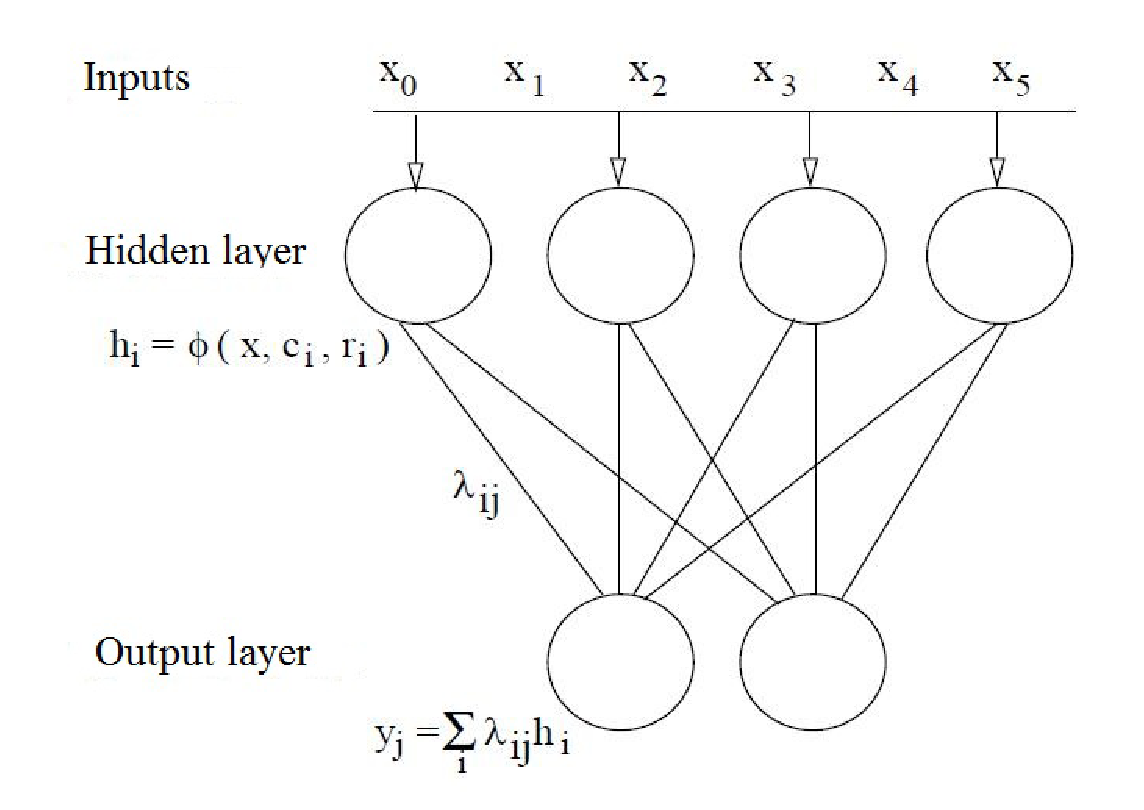
\includegraphics[width=120mm]{rnfbr.eps}
\caption{Radial Basis Function Neural Network. Every neuron in the hidden layer uses a Radial Basis Function ($\phi$) as activation function. This function depends on the input ($x$), the point in the input space where the function is centred ($c_i$), and the width or radius established for the neuron ($r_i$). Weights from hidden to output layers (namely $\lambda_{ij}$) can be efficiently calculated provided that there exist enough training data.} 
\label{fig:rbfnn} 
\end{figure}

\newpage
\clearpage

\begin{figure}[!ht]
\includegraphics[width=120mm]{gausiana.eps}
\caption{Gaussian function: $y=e^{\frac{-||X-C||^2}{2r^2}}$; where $X$ is the input pattern, $C$ is the centre of the function and $r$ is tis width or radius.}
\label{fig:gaussian} 
\end{figure}


\newpage
\clearpage

\begin{figure}[!ht]
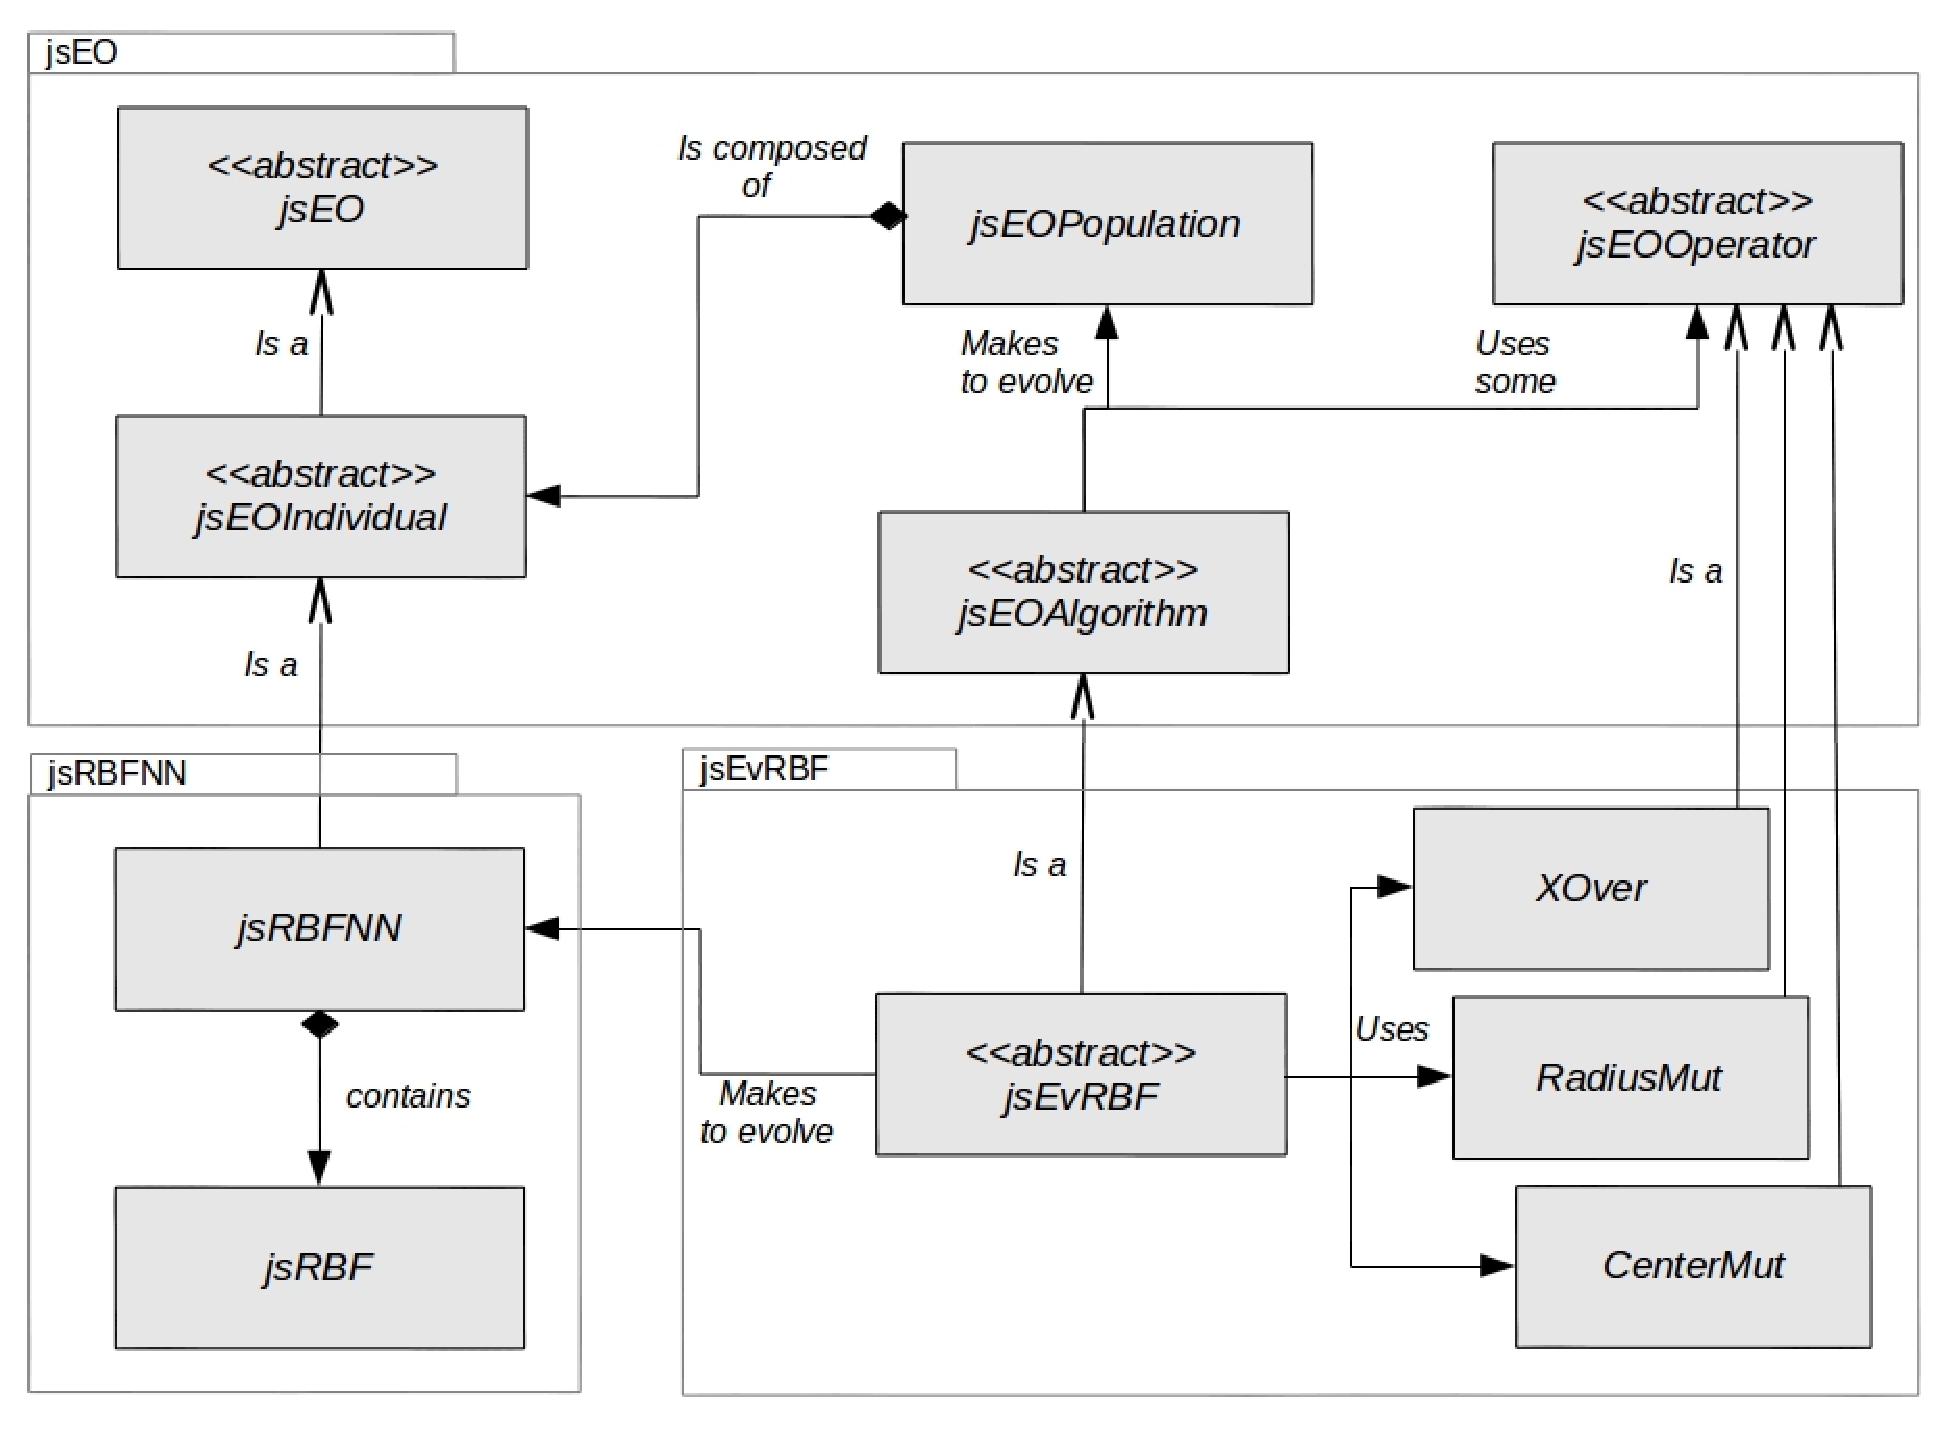
\includegraphics[width=120mm]{class-diagram.eps}
\caption{Class diagram of the jsEvRBF algorithm, showing the way it depends on the jsEO general framework and the jsRBFNN library.}
\label{fig:class_diagram} % Do we need this thing? ~JJ -  I really
                          % like it. BTW, I wish we had realised in EO
                          % that eo wasn't a class, but an Interface ~vrivas
% we did know it was an interface. We used the STL, and in later
% implementation, "traits" to extend it - JJ
\end{figure}

\newpage
\clearpage

\begin{figure}[!ht]
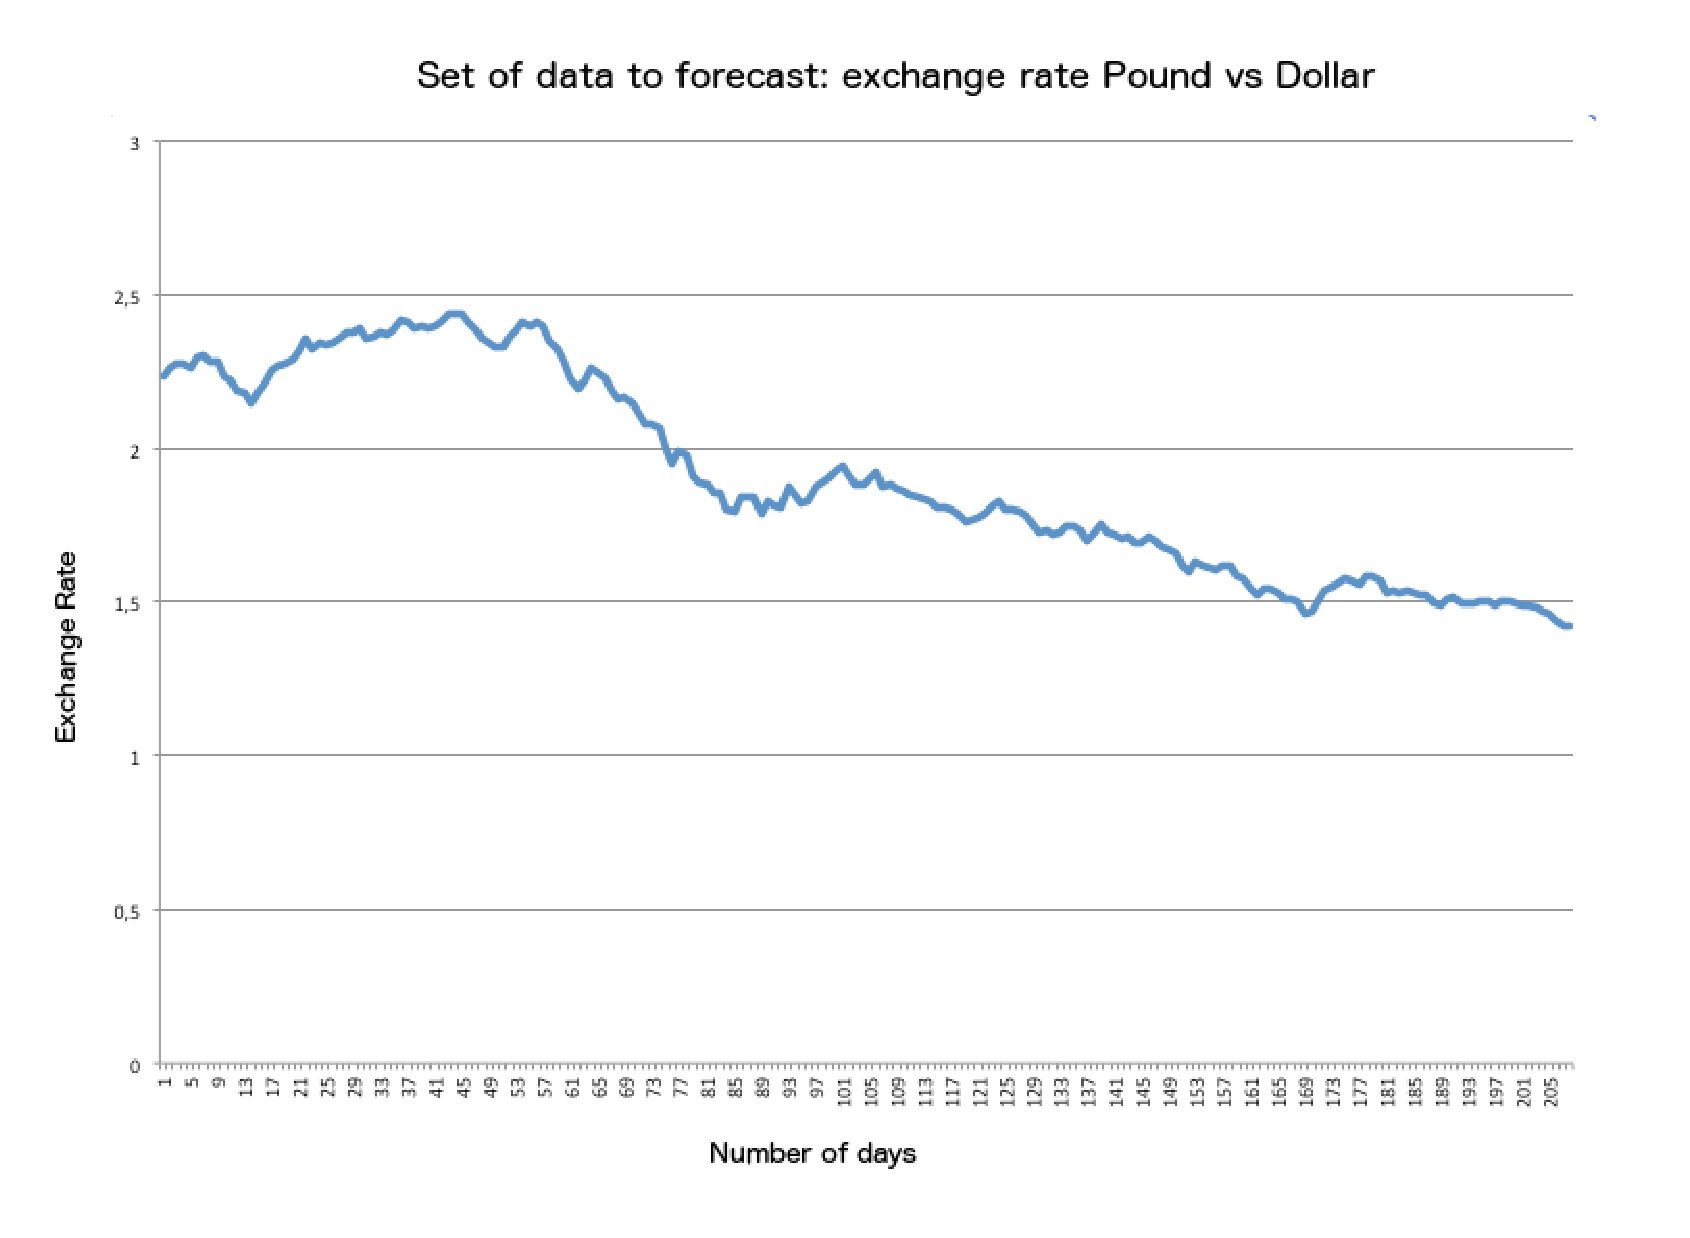
\includegraphics[width=120mm]{time-series.eps}
\caption{Time-series being forecasted in this paper. The data represent the exchange rates between Bristish pound and US dollar from 31 December 1979 to 26 December 1983\cite{Sheta2001}.}
\label{fig:time-series}
\end{figure}


\newpage
\clearpage

\begin{figure}[!ht]
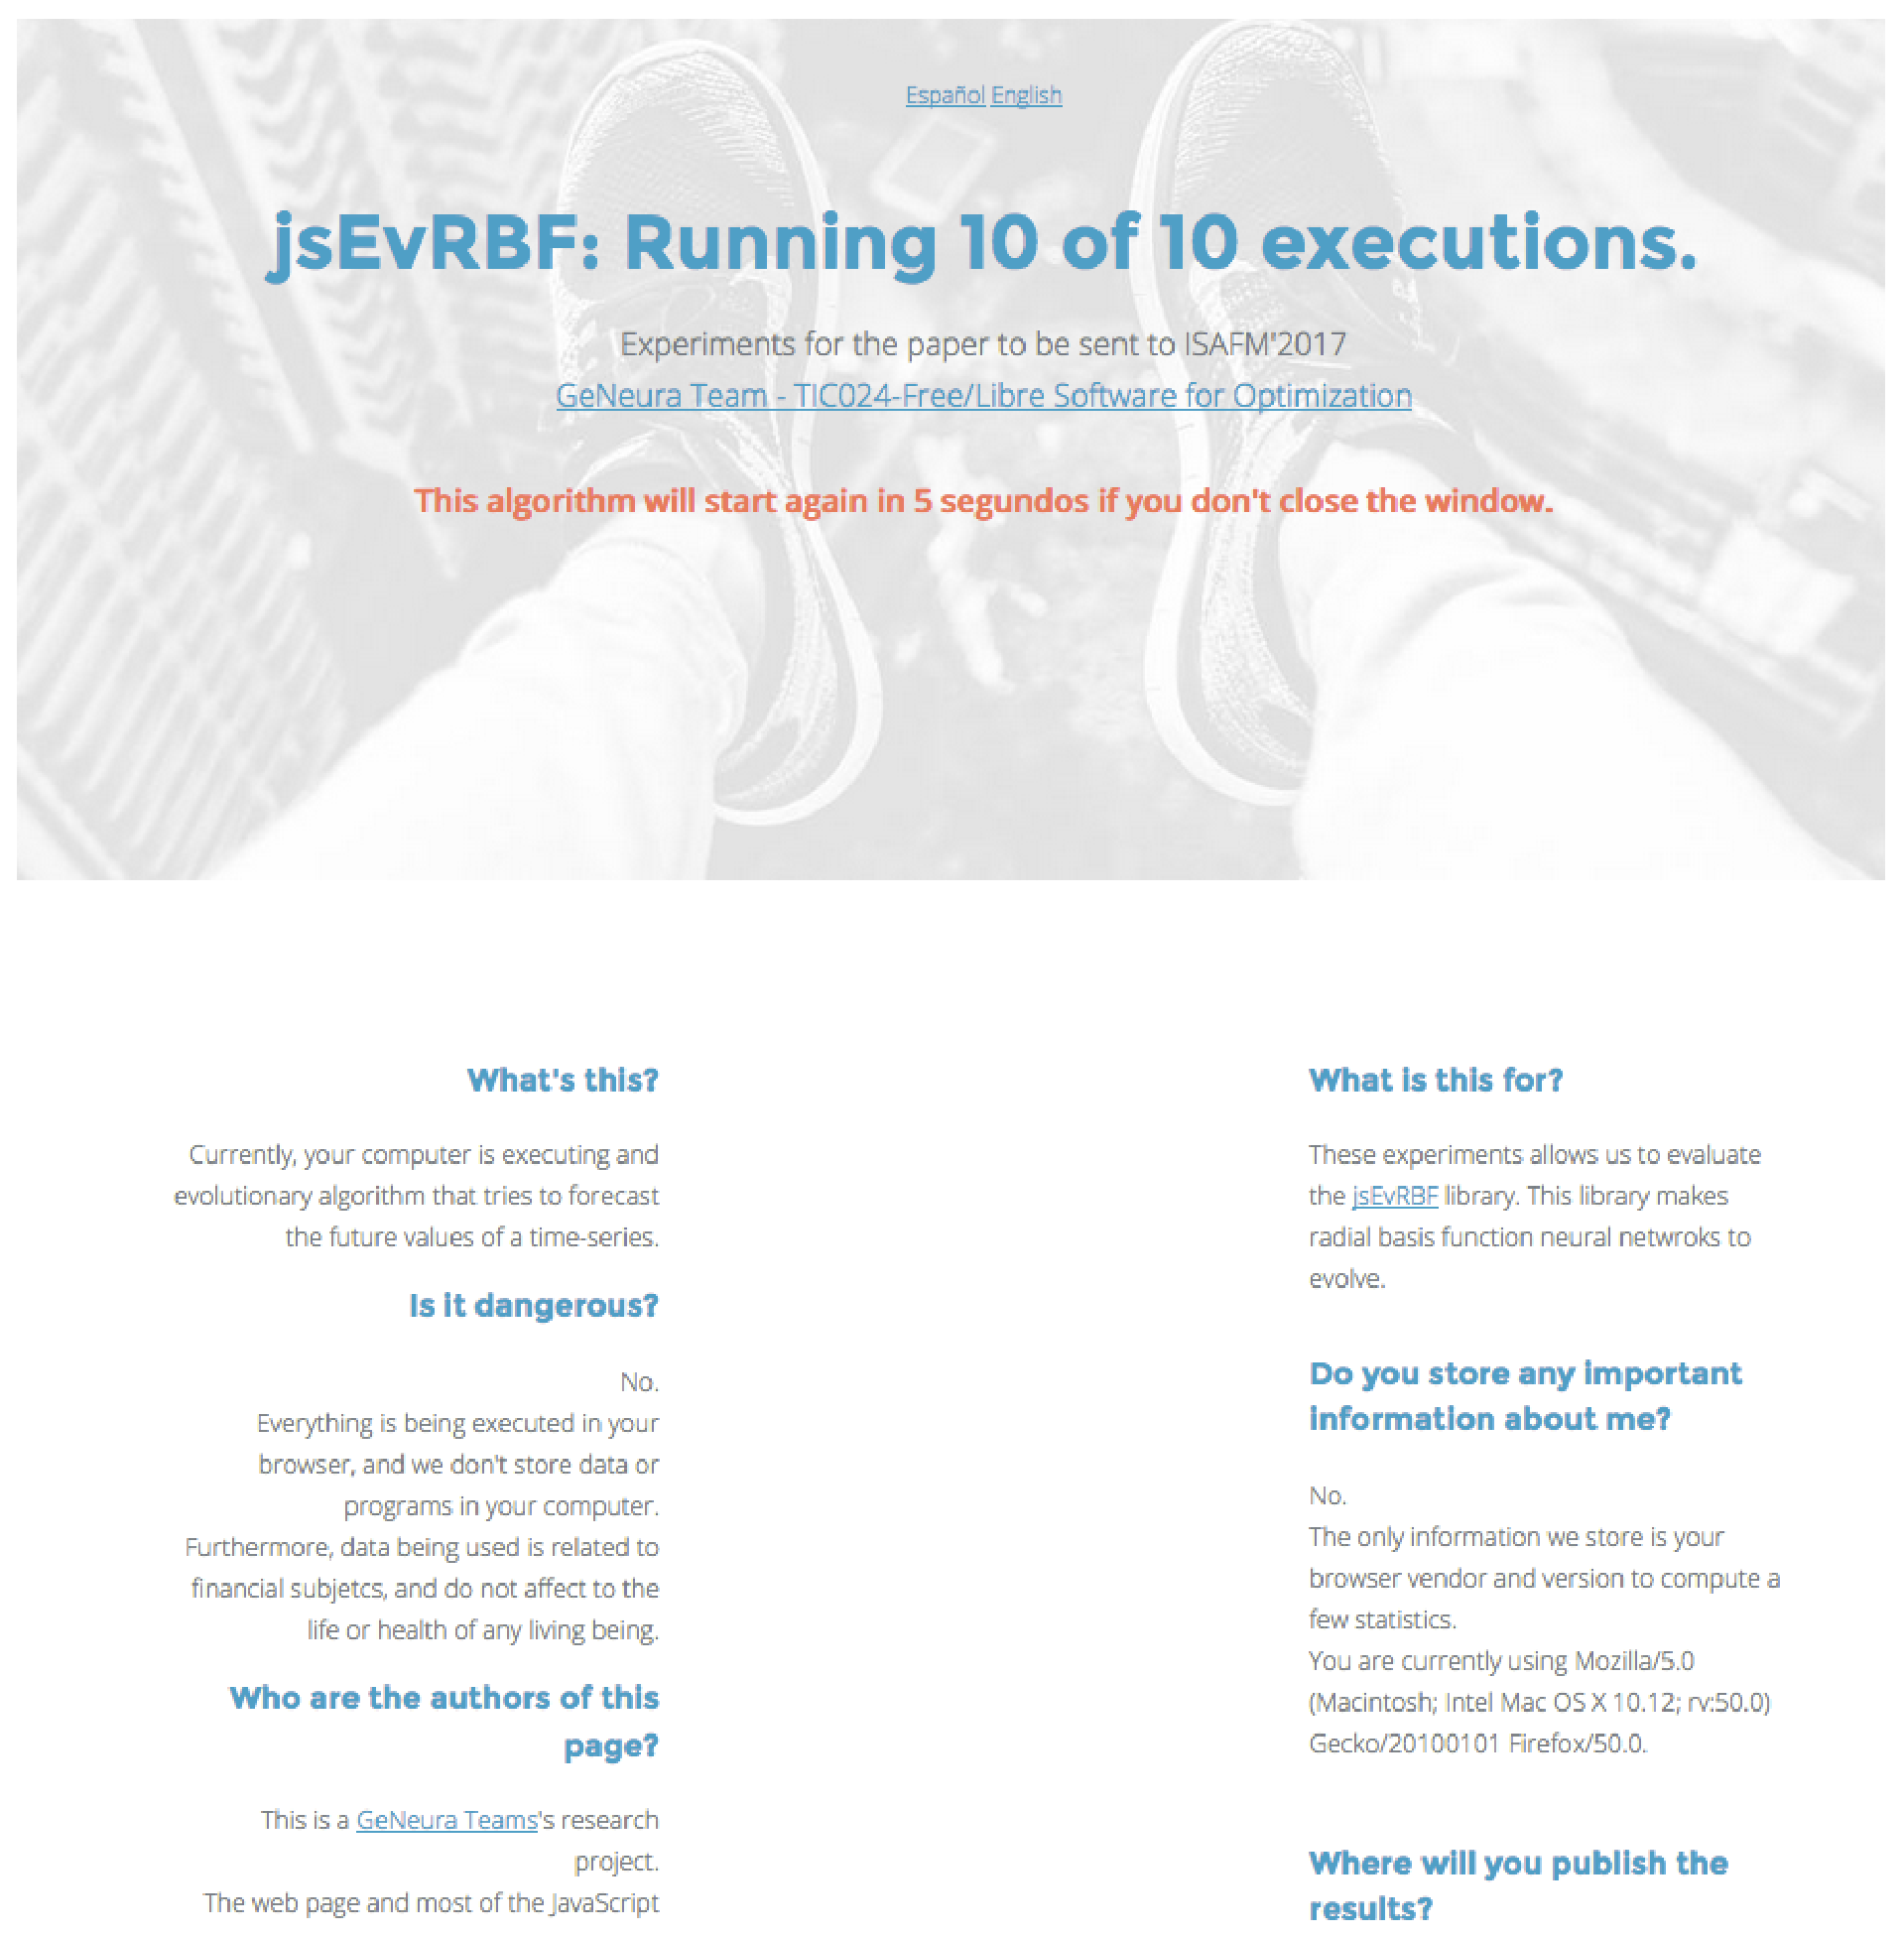
\includegraphics[width=120mm]{example-of-execution-isafm.eps}
\caption{The look of the web page in which the {\em jsEvRBF} algorithm was loaded and executed.}
\label{fig:example-of-execution}
\end{figure}
\newpage
\clearpage


\setlength{\tabcolsep}{10pt}
\begin{table}
\caption{Configuration of parameters for the experiments. The number of samples ({\em trnSamples} and {\em valSamples}) is still approximated since they were randomly chosen in every execution.}
\label{tab:parameters-experiments}
\begin{center}
\begin{tabular}{rr|rr}
{\bf Parameter} & {\bf Value} &
{\bf Parameter} & {\bf Value}\\
\hline
{\em trnSamples} & $\approx 90$ &
{\em valSamples} & $\approx 15$  \\
{\em inputDimension} &   1 &
{\em numNeurons} &  10 \\
{\em popSize} &  15 &
{\em numGenerations} & 10  \\
{\em tournamentSize} &  3 &
{\em replaceRate} &   0.2 \\
{\em xOverRate} &  0.2&
{\em mutRate} &   0.8  \\
{\em mutPower} &  0.5 &
{\em Executions per page load} & 1 \\
\hline
\end{tabular}
\end{center}
\end{table}

% Second one: only one browser, complete executions



\newpage
\clearpage

\setlength{\tabcolsep}{10pt}
\begin{table}
\caption{Operating systems used in the first experiment, the one open to any user. The values indicated the percentage of use of every operating system.}
\label{tab:ooss-first-experiment}
\begin{center}
\begin{tabular}{cc}
{\bf Operating System} & {\bf Use\%} \\
\hline
\bf Android & $\mathbf{54.5\%}$ \\
Windows & $18.2\%$ \\
Mac Os & $18.2\%$ \\
Linux & $9.1\%$ \\
\hline
\end{tabular}
\end{center}
\end{table}


\newpage
\clearpage

\setlength{\tabcolsep}{10pt}
\begin{table}
\caption{Browsers used by participants in the first experiment. The values indicated the percentage of use of each browser.}
\label{tab:browsers-first-experiment}
\begin{center}
\begin{tabular}{cc}
{\bf Browser} & {\bf Use\%} \\
\hline
\bf Chrome & $\mathbf{69.1\%}$ \\
Firefox & $20.0\%$ \\
Safari & $10.9\%$ \\
\hline
\end{tabular}
\end{center}
\end{table}
% Then, the majority of the users are running the faulty algorithm? - HH

\newpage
\clearpage


\setlength{\tabcolsep}{10pt}
\begin{table}
\caption{First experiment: comparison of MSE yielded by the {\em
    jsEvRBF} algorithm and the ones cited in \cite{rivas03:EvRBF}. Row
  {\em jsEvRBF'16} includes the results presented in PAAMS congress,
  while row {\em jsEvRBF'17} belongs to this new set of
  experiments. Errors have been computed over the full set of data.}
\label{tab:comparison-first-experiment}
\begin{center}
\begin{tabular}{lcc}
{\bf Method} & {\bf Average MSE} & {\bf Best MSE} \\
\hline
\bf EvRBF & $\mathbf{6 \times 10^{-4} \pm 2 \times 10^{-4}}$ &$\mathbf{4 \times 10^{-4}}$ \\
MSE-GA & $9 \times 10^{-4}$ & N/A \\
MSE-LSE &  $1 \times 10^{-3}$ & N/A \\
{\em jsEvRBF'17} & $\mathit{2 \times 10^{-3} \pm 5 \times 10^{-3}}$ & $\mathit{6 \times 10^{-4}}$  \\
jsEvRBF'16 & $2 \times 10^{-2} \pm 5 \times 10^{-2}$ & $6 \times10^{-4}$  \\
\hline
\end{tabular}
% Are you sure this is correct? Standard deviation two orders of
% magnitude bigger than value? 0.002 +- 0.8? Really? - JJ
% No... it's a mistake when copying from console to latex... :/
\end{center}
\end{table}

\newpage
\clearpage


\setlength{\tabcolsep}{10pt}
\begin{table}
\caption{Second experiment: browsers used to run the {\em jsEvRBF}
  algorithm.}
% Different computers or different virtual machines in the same
% computer? If they are different computers, what are you comparing?
% The random number generator? - JJ
% I tested all that I had close to me - Victor.
\label{tab:browsers-second-experiment}
\begin{center}
\begin{tabular}{lcc}
{\bf Browser} & {\bf Version} & {\bf Operating System} \\
\hline
Chrome & 55.0.2883.87 & Windows \\
Chrome & 55.0.2883.95 & Mac OS \\
Chromium\footnote{The open-source project behind Chrome} & 51.0.2704.79 & Linux \\
Edge & 14.14393.0.0 & Windows \\
Firefox & 47.0 & Linux \\
Firefox & 50.1.0 & Linux \\
Firefox & 50.1.0 & Mac Os \\
Safari & 10.0.2 & Mac OS \\
\hline
\end{tabular}
\end{center}
\end{table}



\newpage
\clearpage

\setlength{\tabcolsep}{10pt}
\begin{table}
\caption{Second experiment: MSE and standard deviation yielded by the different browsers used to run the {\em jsEvRBF} algorithm. Values are averaged over the number of valid executions\protect\footnotemark.}
\label{tab:results-per-browser-second-experiment}
\begin{center}
\begin{tabular}{lcc}
{\bf Browser}	 & \bf{MSE} 	$\mathbf{\pm}$ {\bf STD.DEV}	 & 	{\bf Valid Executions}	 \\
\hline
\bf Chromium 51.0.2704.79 (Linux)	 & 	$\mathbf{7.4\times10^{-4} \pm 	1.6 \times 10^{-4}}$	 & 	$\mathbf{5}$	 \\
Firefox 47.0 (Linux)	 & 	$8.5 \times 10^{-4}	 \pm 	1.4 \times 10^{-4}$	 & 	$10$	 \\
Firefox 50.1.0 (Mac OS)	 & 	$8.7 \times 10^{-4}	 \pm 	3.0 \times 10^{-4}$	 & 	$10$	 \\
Firefox 50.1.0 (Linux)	 & 	$9.2 \times 10^{-4}	 \pm 	3.1 \times 10^{-4}$	 & 	$10$	 \\
Chrome 55.0.2883.87 (Windows)	 & 	$1.2 \times 10^{-3}	 \pm 	7.3 \times 10^{-4}$	 & 	$7$	 \\
Chrome 55.0.2883.95 (Mac OS)	 & 	$1.2 \times 10^{-3}	 \pm 	5.2 \times 10^{-4}$	 & 	$4$	 \\
Edge 14.14393 (Windows)	 & 	$2.0 \times 10^{-2}	 \pm	2.2 \times 10^{-2}$	 & 	$10$	 \\
Safari 10.0.2 (Mac OS)	 & 	$6.0 \times 10^{-2}	\pm 	8.9 \times 10^{-2}$	 & 	$10$	 \\

\hline
\end{tabular}
\end{center}
\end{table}
\footnotetext{The number of valid executions should have been $10$ for
  all browsers, but it is different for Chromium and Chrome browsers,
  since there seems to be a bug that makes these browsers yield {\em NaN} when training the neural nets in a few executions.}


\newpage
\clearpage

\setlength{\tabcolsep}{10pt}
\begin{table}
\caption{Ranking of browsers according to Friedman's test. Values in column $\chi^2$ indicate the degrees of freedom for the $\chi^2$ distribution followed by the different solutions provided by each client: the lowset this value, the better the position in the ranking. }
\label{tab:friedman-results}
\begin{center}
\begin{tabular}{clcc}
\bf Position & {\bf Browser}	 &  {$\mathbf{\chi^2}$} 	 \\
\hline
\bf 1 & \bf Firefox 50.1.0 (Mac OS)	& $\mathbf{2.00}$\\
2 & Firefox 47.0 (Linux)	& $2.70$\\
3 & Firefox 50.1.0 (Linux)	& $3.00$\\
4 & Chromium51.0.2704.79 (Linux)	& $4.75$\\
5 & Chrome 55.0.2883.87 (Windows)	& $5.30$\\
6 & Edge 14.14393	& $5.60$\\
7 & Safari 10.0.2 (Mac OS)	& $5.80$\\
8 & Chrome 55.0.2883.95 (Mac OS)	& $6.85$\\
\hline
\end{tabular}
\end{center}
\end{table}

\newpage
\clearpage

\setlength{\tabcolsep}{10pt}
\begin{table}
\caption{Results of the Holms procedure. Control browser is Firefox 50.1.0 under Mac OS; the null hypothesis is rejected when it does not exist significant differences between the browser being considered in every row and the control browser. Column $\rho$ indicates the adjusted $\rho-value$ for every browser with respect to the control browser. Column  $\alpha/i$ represents the alpha level used to accept or reject the null hypothesis. As $\alpha$ has been established to $0.05$, the null hypothesis is rejected when $\rho<\alpha/i$.}
\label{tab:holm-results}
\begin{center}
\begin{tabular}{cp{45mm}ccl}
\bf i & \bf Control browser: \newline Firefox 50.1.0 (Mac OS)	&	$\mathbf{\rho}$	&	\bf $\mathbf{\alpha/i}$	&	\bf Null hypothesis	\\
\hline
\bf 1 & \bf Firefox 50.1.0 (Linux)		&	\bf 0.00003	&	\bf 0.00714	&	\bf Rejected	\\
\bf 2 & \bf Firefox 47.0 (Linux)			&	\bf 0.00140	&	\bf 0.00833	&	\bf Rejected	\\
\bf 3 & \bf Chromium 51.0.2704.79 (Linux)	&	\bf 0.00259	&	\bf 0.01000	&	\bf Rejected	\\
\bf 4 & \bf Chrome 55.0.2883.87 (Windows)	&	\bf 0.00811	&	\bf 0.01250	&	\bf Rejected	\\
5 & Edge 4.14393				&	0.01992	&	0.01667	&	Non Rejected	\\
6 & Safari 10.0.2 (Mac OS)		&	0.71500	&	0.02500	&	Non Rejected	\\
7 & Chrome 55.0.2883.95 (Mac OS)	&	0.71500	&	0.05000	&	Non Rejected	\\
\hline
\end{tabular}
\end{center}
\end{table}

\end{document}
